%!TEX root = ../thesis.tex
%*******************************************************************************
%****************************** Second Chapter *********************************
%*******************************************************************************

\chapter{Deep learning for computational biology}

\ifpdf
    \graphicspath{{Chapter2/Figs/Raster/}{Chapter2/Figs/PDF/}{Chapter2/Figs/}}
\else
    \graphicspath{{Chapter2/Figs/Vector/}{Chapter2/Figs/}}
\fi

\section{Introduction}
Machine learning methods are general-purpose approaches to learn functional relationships from data without the need to define them a priori~\citep{hastie_elements_2005,michalski_machine_2013,murphy_machine_2012}. In computational biology, their appeal is the ability to derive predictive models without a need for strong assumptions about underlying mechanisms, which are frequently unknown or insufficiently defined. As a case in point, the most accurate prediction of gene expression levels is currently made from a broad set of epigenetic features using sparse linear models~\citep{cheng_statistical_2011,karlic_histone_2010} or random forests~\citep{li_using_2015}; how the selected features determine the transcript levels remains an active research topic. Predictions in genomics~\citep{libbrecht_machine_2015,martens_predicting_2016}, proteomics~\citep{swan_application_2013}, metabolomics~\citep{kell_metabolomics_2005}, or sensitivity to compounds~\citep{eduati_prediction_2015} all rely on machine learning approaches as a key ingredient.

Most of these applications can be described within the canonical machine learning workflow, which involves four steps: data cleaning and pre-processing, feature extraction, model fitting, and evaluation (\autoref{fig:figure1}~(A)). It is customary to denote one data sample, including all covariates and features as input $x$ (usually a vector of numbers), and label it with its response variable or output value $y$ (usually a single number) when available.

\begin{figure}[htbp!]
\centering
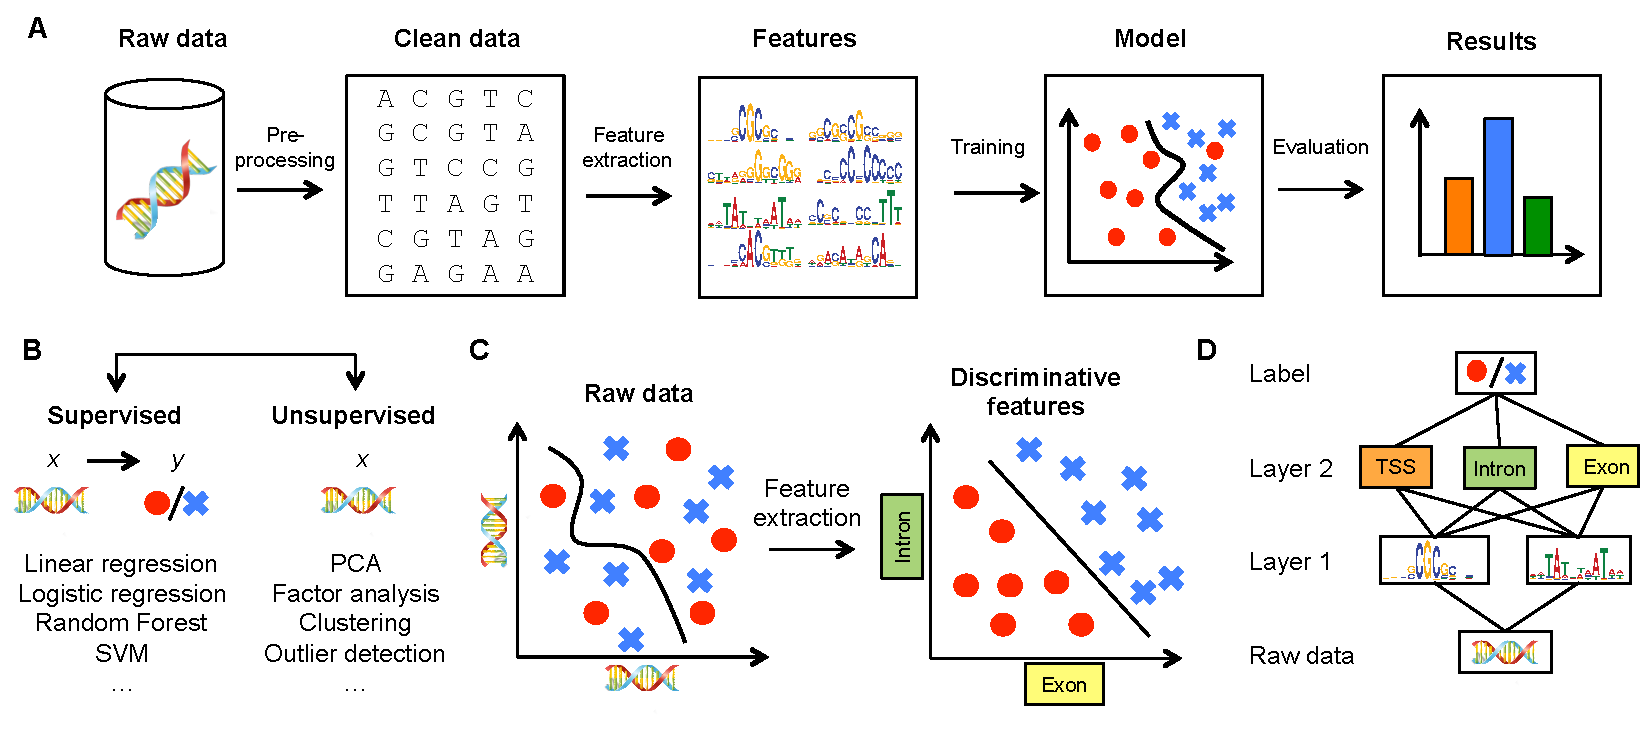
\includegraphics[width=1.0\textwidth]{figure1}
\caption[Machine learning and representation learning.]{Machine learning and representation learning. (A) The classical machine learning workflow can be broken down into four steps: data pre-processing, feature extraction, model learning, and model evaluation. (B) Supervised machine learning methods relate input features $x$ to an output label $y$, whereas unsupervised method learn factors about $x$ without observed labels. (C) Raw input data are often high dimensional and related to the corresponding label in a complicated way, which is challenging for many classical machine learning algorithms (left plot). Alternatively, higher-level features extracted using a deep model may be able to better discriminate between classes (right plot). (D) Deep networks use a hierarchical structure to learn increasingly abstract feature representations from the raw data.}
\label{fig:figure1}
\end{figure}

A supervised machine learning model aims to learn a function $f(x)=y$ from a list of training pairs $(x_1,y_1), (x_2,y_2),\ldots$ for which data are recorded (\autoref{fig:figure1}~(B)). One typical application in biology is to predict the viability of a cancer cell line when exposed to a chosen drug~\citep{eduati_prediction_2015,menden_machine_2013}. The input features $x$ would capture somatic sequence variants of the cell line, chemical makeup of the drug, and its concentration, which together with the measured viability (output label $y$) can be used to train a support vector machine, a random forest classifier or a related method (functional relationship $f$). Given a new cell line (unlabelled data sample $x^*$) in the future, the learnt function predicts its survival (output label $y^*$) by calculating $f(x^*)$, even if $f$ resembles more of a black box, and its inner workings of why particular mutation combinations influence cell growth are not easily interpreted. Both regression (where $y$ is a real number), and classification (where $y$ is a categorical class label) can be viewed in this way. As a counterpart, unsupervised machine learning approaches aim to discover patterns from the data samples $x$ itself, without the need for output labels $y$. Methods such as clustering, principal components analysis, and outlier detection are typical examples of unsupervised models applied to biological data.

The inputs $x$, calculated from the raw data, represent what the model `sees about the world', and their choice is highly problem specific (\autoref{fig:figure1}~(C)). Deriving most informative features is essential for performance, but the process can be labour-intensive and requires domain knowledge. This bottleneck is especially limiting for high dimensional data; even computational feature selection methods do not scale to assess the utility of vast number of possible input combinations. A major recent advance in machine learning is automating this critical step by learning a suitable representation of the data with deep artificial neural networks~\citep{bengio_representation_2013,lecun_deep_2015,schmidhuber_deep_2015} (\autoref{fig:figure1}~(D)). Briefly, a deep neural network takes the raw data at the lowest (input) layer, and transforms them into increasingly abstract feature representations by successively combining outputs from the preceding layer in a data-driven manner, encapsulating highly complicated functions in the process (Box 1). Deep learning is now one of the most active fields in machine learning and has been shown to improve performance in image- and speech recognition~\citep{deng_deep_2015,graves_generating_2013,hinton_deep_2012,krizhevsky_imagenet_2012,zeiler_visualizing_2014}, natural language understanding~\citep{bahdanau_neural_2014,lipton_critical_2015,sutskever_sequence_2014,xiong_dynamic_2016}, and most recently, in computational biology~\citep{alipanahi_predicting_2015,dahl_multi-task_2014,eickholt_dndisorder:_2013,kelley_basset:_2016,leung_deep_2014,sonderby_protein_2014,wang_chromatin_2015,zhou_predicting_2015}.

The potential of deep learning in high throughput biology is clear: in principle, it allows to better exploit the availability of increasingly large and high-dimensional datasets (e.g. from DNA sequencing, RNA measurements, flow cytometry, or automated microscopy) by training complex networks with multiple layers that capture their internal structure (\autoref{fig:figure1}~(C)). The learned networks discover high-level features, improve performance over traditional models, increase interpretability and provide additional understanding about the structure of the biological data.

In this review, we discuss recent and forthcoming applications of deep learning, with a focus on applications in regulatory genomics and biological image analysis. The goal of this review is not to provide comprehensive background on all technical details, which can be found in more specialized literature~\citep{bengio_practical_2012,bengio_representation_2013,deng_deep_2014,goodfellow_deep_2016,schmidhuber_deep_2015}. Instead, we aim to provide practical pointers and the necessary background to get started with deep architectures, review current software solutions, and give recommendations for applying them to data. The applications we cover are deliberately broad to illustrate differences and communalities between approaches; reviews focusing on specific domains can be found elsewhere~\citep{gawehn_deep_2016,leung_machine_2016,mamoshina_applications_2016,park_deep_2015}. Finally, we discuss both the potential and possible pitfalls of deep learning and contrast these methods to traditional machine learning and classical statistical analysis approaches.

\subsection{Artificial neural networks}
An artificial neural network, initially inspired by neural networks in the brain \citep{farley_simulation_1954,mcculloch_logical_1943,rosenblatt_perceptron:_1958} consists of layers of interconnected compute units (neurons). In the canonical configuration, the network receives data in an input layer, which are then transformed in a nonlinear way through multiple hidden layers, before final outputs are computed in the output layer (\autoref{fig:figure2}~(A)). Neurons in a hidden or output layer are connected to all neurons of the previous layer. Each neuron computes a weighted sum of its inputs, and applies a nonlinear activation function to calculate its output (\autoref{fig:figure2}~(B)). The most popular activation function is the Rectified linear unit (ReLU, (\autoref{fig:figure2}~(B)), since it allows faster learning compared to alternatives (e.g. sigmoid or tanh unit) \citep{glorot_deep_2011}. The depth of a neural network corresponds to the number of hidden layers, and the width to the maximum number of neurons in one of its layers. As it became possible to train networks with larger numbers of hidden layers, artificial neural networks were rebranded to ``deep networks''.

The weights between neurons are free parameters that capture the model's representation of the data, and are learned from input/output samples. Learning minimizes a loss function that measures the fit of the model output to the true label of a sample (\autoref{fig:figure2}~(A), bottom). This minimization is challenging, since the loss function is high dimensional and non-convex, similar to a landscape with many hills and valleys (\autoref{fig:figure2}~(C)). It took several decades before the backward propagation algorithm was first applied to compute a loss function gradient via chain rule for derivatives \citep{rumelhart_learning_1988}, ultimately enabling efficient training of neural networks using stochastic gradient descent. During learning, the predicted label is compared with the true label to compute a loss for the current set of model weights. The loss is then backward propagated through the network to compute the gradients of the loss function and update (\autoref{fig:figure2}~(A)). While learning in deep neural networks remains an active area of research, existing software packages (Table 1) can already be applied without knowledge of the mathematical details involved.

Alternative architectures to such fully connected feedforward networks have been developed for specific applications, which differ in the way neurons are arranged. These include convolutional neural networks, which are widely used for modelling images (Box 2), recurrent neural networks for sequential data \citep{lipton_critical_2015,sutskever_training_2013}, or restricted Boltzmann machines \citep{hinton_practical_2012,salakhutdinov_efficient_2010} and autoencoders \citep{alain_regularized_2012,hinton_reducing_2006,kingma_auto-encoding_2013} for unsupervised learning. The choice of network architecture and other parameters can be made in a data driven and objective way by assessing the model performance on a validation dataset.


\begin{figure}[htbp!]
\centering
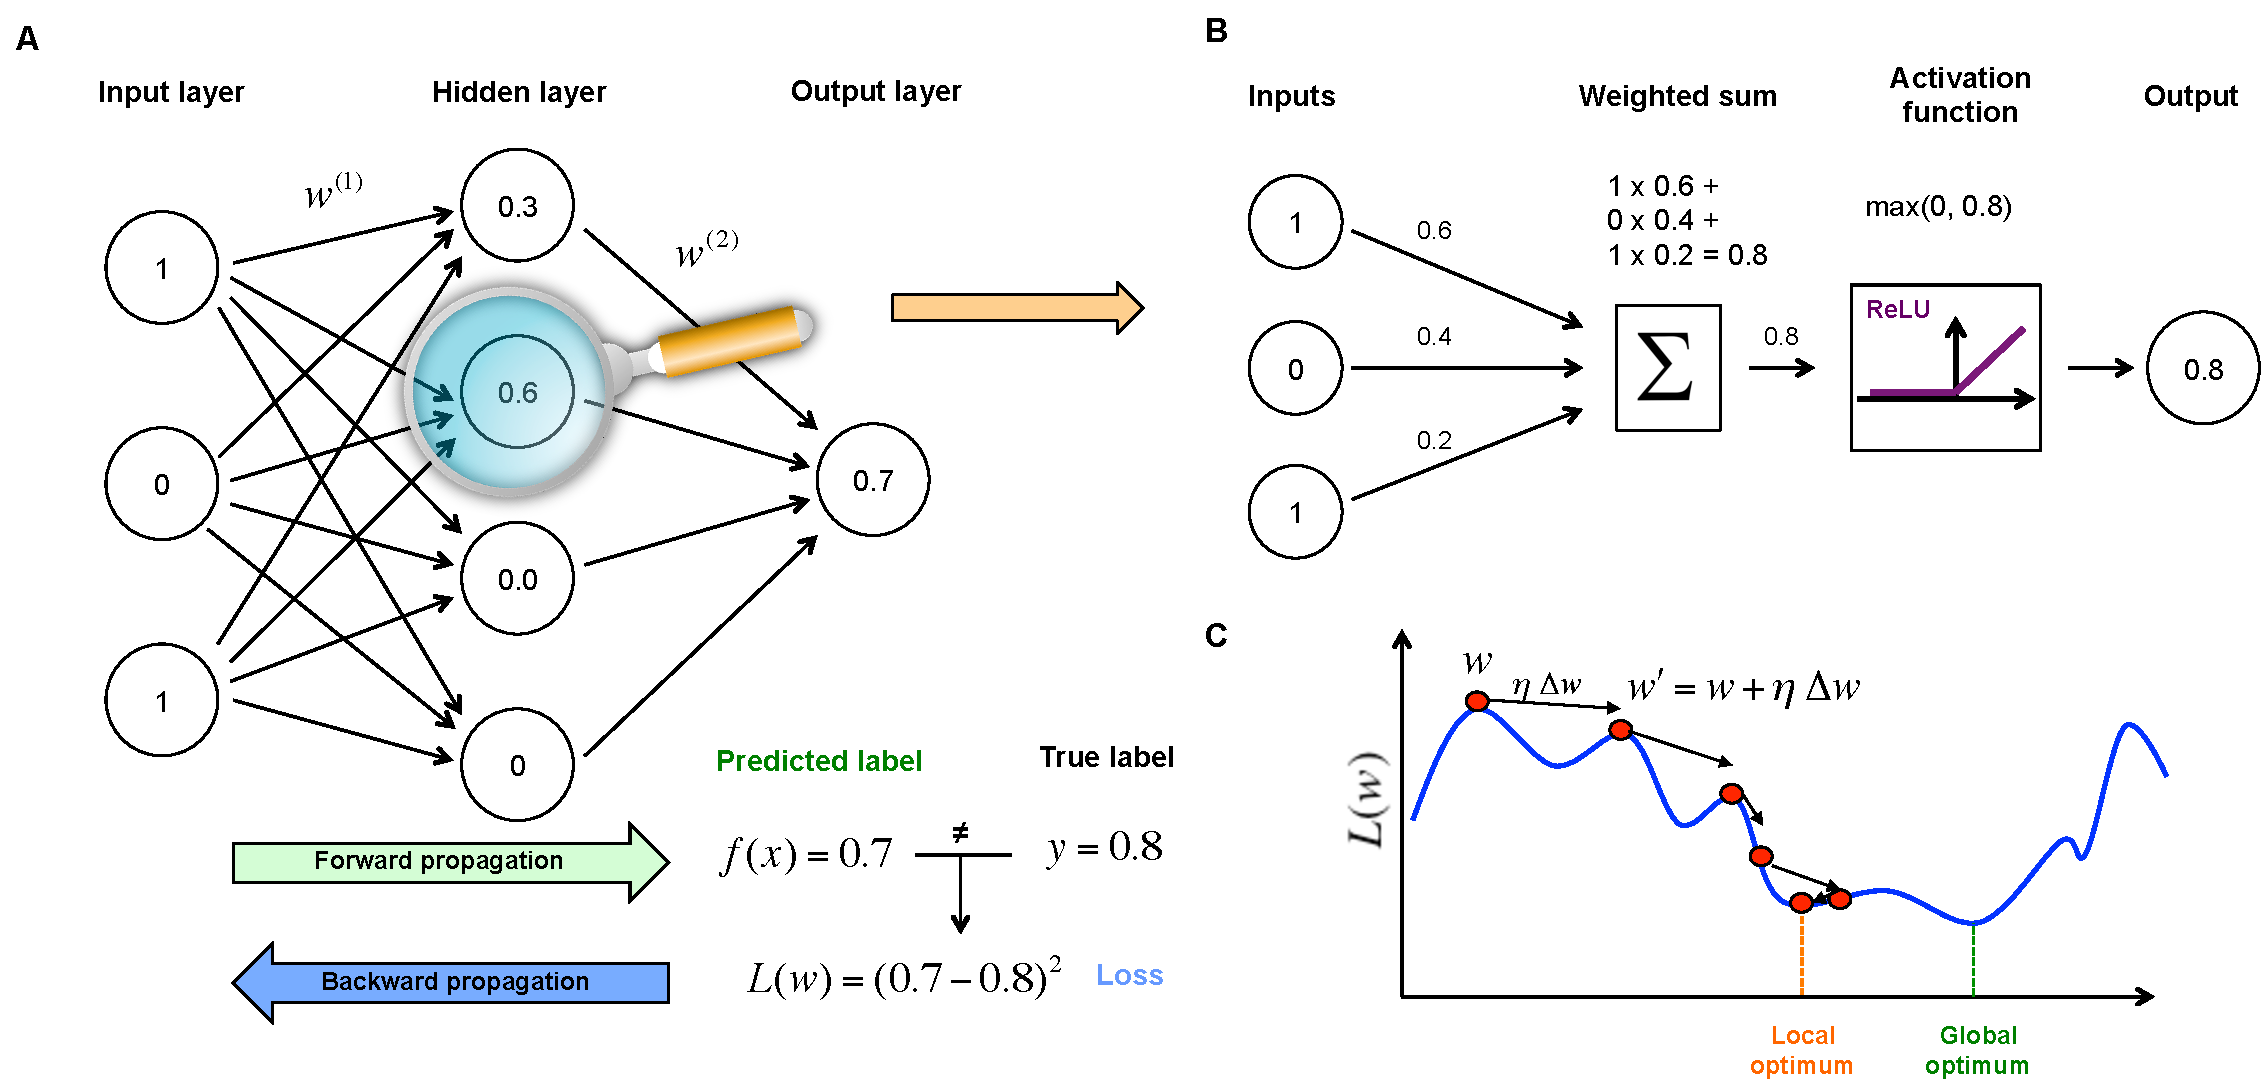
\includegraphics[width=1.0\textwidth]{figure2}
\caption[Building blocks and learning principles of a neural network.]{Building blocks and learning principles of a neural network. (A) Fully connected feedforward neural network with one input layer, hidden layer, and output layer.  Each layer $i$ consists of neurons which are connected to all neurons of the previous layer with weights $w(i)$. Given input $x$, neuron activations are calculated and forward propagated to the output layer to obtain a prediction $f(x)$. (B) Zoom-in view into one neuron, which computes the weighted sum of its inputs and applies a rectification function that thresholds negative signals to $0$, and passes through positive signal. (C) Gradient-based optimization of the loss function $L(w)$. In each step, the current weight vector (red dot) is moved along the direction of steepest descent $\Delta w$ (direction arrow) by learning rate $\eta$ (length of vector). Decaying the learning rate over time allows to explore different domains of the loss function by jumping over valleys at the beginning of the training (left side), and fine-tune parameters with smaller learning rates in later stages of the model training.}
\label{fig:figure2}
\end{figure}


\section{Deep learning for regulatory genomics}
Conventional approaches for regulatory genomics relate sequence variation to changes in molecular traits. One approach is to leverage variation between genetically diverse individuals to map quantitative trait loci (QTL). This principle has been applied to identify regulatory variants that affect gene expression levels \citep{montgomery_transcriptome_2010,pickrell_understanding_2010}, DNA methylation \citep{bell_dna_2011,gibbs_abundant_2010}, histone marks \citep{grubert_genetic_2015,waszak_population_2015}, and proteome variation \citep{albert_genetics_2014,battle_genomic_2015,parts_heritability_2014,vincent_stacked_2010} (\autoref{fig:figure3}~(A)). Better statistical methods have helped to increase the power to detect regulatory QTLs \citep{kang_accurate_2008,parts_joint_2011,rakitsch_modelling_2016,stegle_bayesian_2010}, however any mapping approach is intrinsically limited to variation that is present in the training population. Thus, studying effects of rare mutations in particular requires extremely large datasets.

An alternative is to train models that use variation between regions within a genome (Fig 3A). Splitting the sequence into windows centred on the trait of interest gives rise to tens of thousands of training examples for most molecular traits even when using a single individual. Even with large datasets, predicting molecular traits from DNA sequence is challenging due to multiple layers of abstraction between effect of individual DNA variants and the trait of interest, as well as the dependence of the molecular traits on a broad sequence context and interactions with distal regulatory elements.

The value of deep neural networks in this context is twofold. First, classical machine learning methods cannot operate on the sequence directly, and thus require predefining features that can be extracted from sequence based on prior knowledge (e.g. the presence of absence of single-nucleotide variants (SNVs), k-mer frequencies, motif occurrences, conservation, known regulatory variants, or structural elements). Deep neural networks can help circumventing the manual extraction of features by learning them from data. Second, because of their representational richness, they can capture nonlinear dependencies in the sequence, interaction effects, and span wider sequence context at multiple genomic scales. Attesting to their utility, deep neural networks have been successfully applied to predict splicing activity \citep{leung_deep_2014,xiong_human_2015}, specificities of DNA- and RNA binding proteins \citep{alipanahi_predicting_2015}, or epigenetic marks and to study the effect of DNA sequence alterations \citep{kelley_basset:_2016,zhou_predicting_2015}.

\subsection{Early applications of neural networks in regulatory genomics}
The first successful applications of neural networks in regulatory genomics replaced a classical machine learning approach with a deep model, without changing the input features. For example, \citeauthor{xiong_human_2015} considered a fully connected feedforward neural network to predict the splicing activity of individual exons. The model was trained using more than $1,000$ pre-defined features extracted from the candidate exon and adjacent introns. Despite the relatively low number of 10,700 training samples in combination with the model complexity, this method achieved substantially higher prediction accuracy of splicing activity compared to simpler approaches, and in particular was able to identify rare mutations implicated in splicing misregulation.

\subsection{Convolutional designs}
More recent work using convolutional neural networks (CNNs) allowed direct training on the DNA sequence, without the need to define features \citep{alipanahi_predicting_2015,angermueller_accurate_2017,kelley_basset:_2016,zhou_predicting_2015}. The CNN architecture allows to greatly reduce the number of model parameters compared to a fully connected network by applying convolutional operations to only small regions of the input space and by sharing parameters between regions. The key advantage resulting from this approach is the ability to directly train the model on larger sequence windows (Box 2, \autoref{fig:figure3}~(B), \autoref{fig:figure4}).

\citeauthor{alipanahi_predicting_2015} considered convolutional network architectures to predict specificities of DNA- and RNA binding proteins \citep{alipanahi_predicting_2015}. Their DeepBind model outperformed existing methods, was able to recover known and novel sequence motifs, and could quantify the effect of sequence alterations and identify functional SNVs. A key innovation that enabled training the model directly on the raw DNA sequence was the application of a one-dimensional convolutional layer. Intuitively, the neurons in the convolutional layer scan for motif sequences and combinations thereof, similar to conventional position-weight matrices \citep{stormo_use_1982}. The learning signal from deeper layers informs the convolutional layer which motifs are most relevant. The motifs recovered by the model can then be visualized as heatmaps or sequence logos (\autoref{fig:figure3}~(D)).

\subsection{In silico prediction of mutation effects}
An important application of deep neural networks trained on the raw DNA sequence is to predict the effect of mutations in silico. Such model-based assessments of the effect of sequence changes complement methods based on QTL mapping, and can in particular help to uncover regulatory effects of rare SNVs or to fine-map likely causal genes. An intuitive approach for visualizing such predicted regulatory effects are mutation maps \citep{alipanahi_predicting_2015}, whereby the effect of all possible mutations for a given input sequence is represented in a matrix view (\autoref{fig:figure3}~(E)). The authors could further reliably identify deleterious SNVs, by training an additional neural network with predicted binding scores for a wild type and mutant sequence (\autoref{fig:figure3}~(C)).

\begin{figure}[htbp!]
\centering
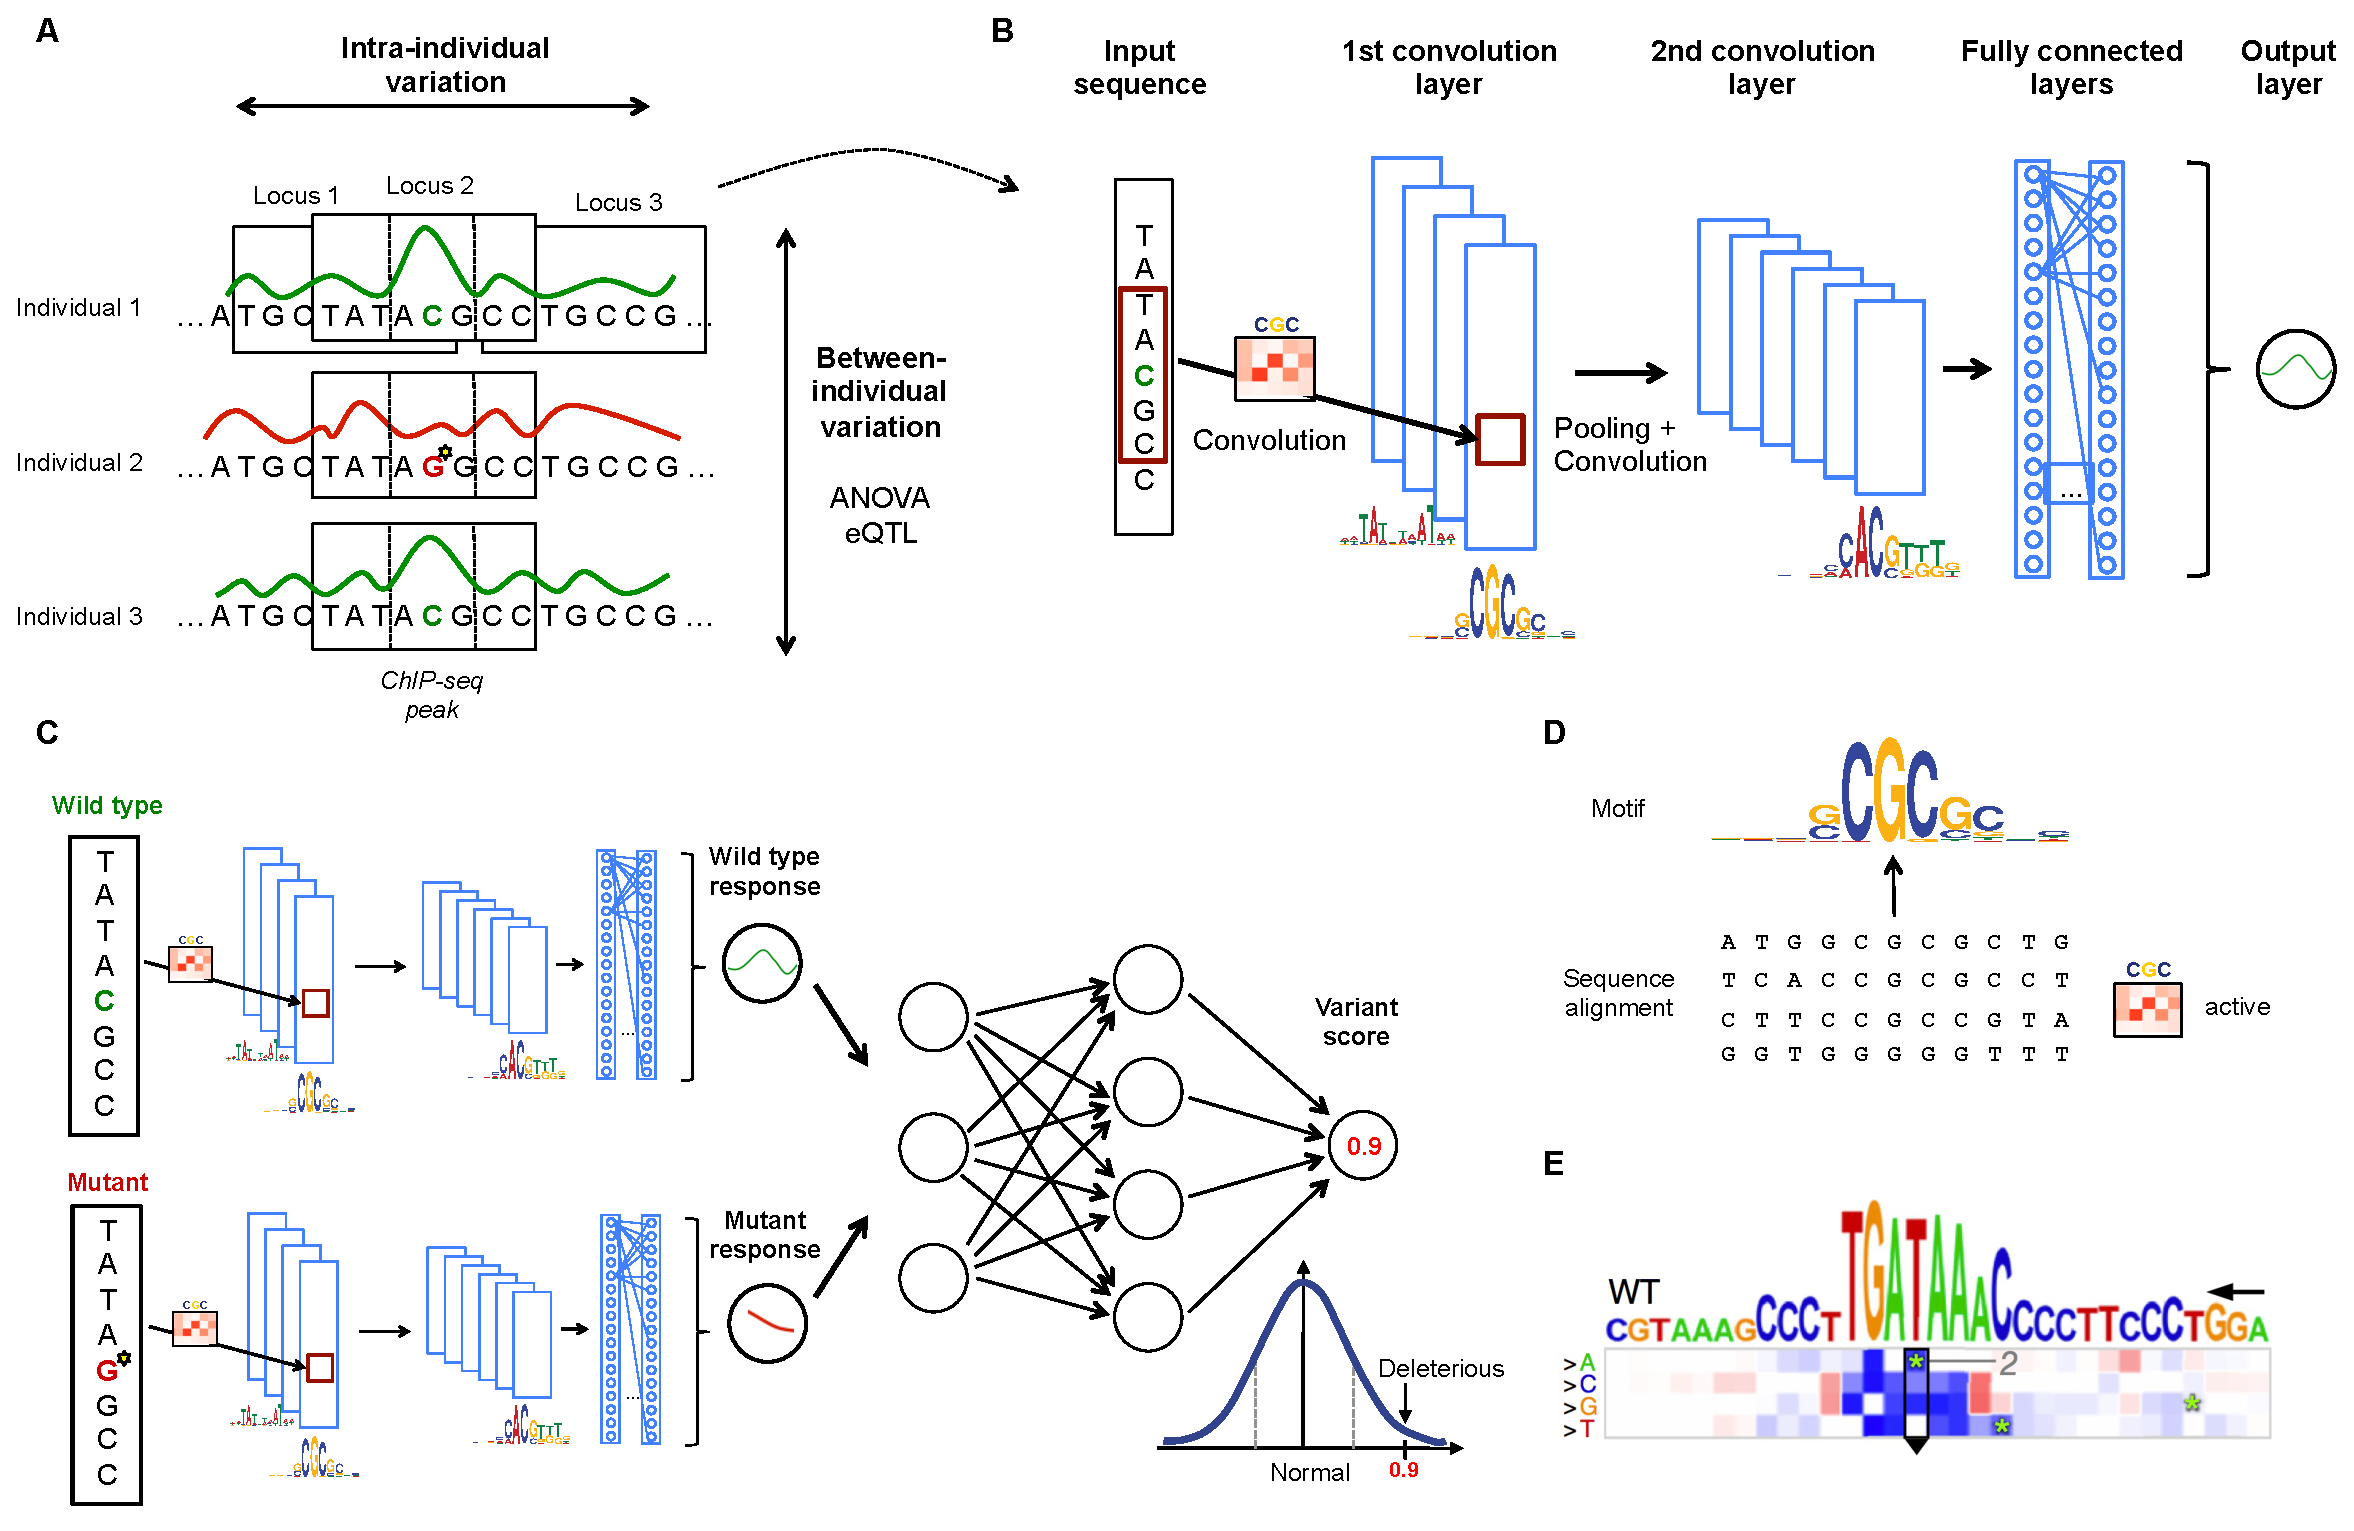
\includegraphics[width=1.0\textwidth]{figure3}
\caption[Principles of using neural networks for predicting molecular traits from DNA sequence.]{Principles of using neural networks for predicting molecular traits from DNA sequence. (A) DNA sequence and the molecular response variable along the genome for three individuals. Conventional approaches in regulatory genomics consider variations between individuals, whereas deep learning allows exploiting intra-individual variations by tiling the genome into sequence DNA windows centred on individual traits, resulting in large training datasets from a single sample. (B) One-dimensional convolutional neural network for predicting a molecular trait from the raw DNA sequence in a window. Filters of the first convolutional layer (example shown on the edge) scan for motifs in the input sequence. Subsequent pooling reduces the input dimension, and additional convolutional layers and can model interactions between motifs in the previous layer. (C) Response variable predicted by the neural network shown in (B) for a wild type and mutant sequence is used as input to an additional neural network that predicts a variant score and allows to discriminate normal from deleterious variants. (D) Visualization of a convolutional filter by aligning genetic sequences that maximally activate the filter and creating a sequence motif. (E) Mutation map of a sequence window. Rows correspond to the four possible base pair substitutions, columns to sequence positions. The predicted impact of any sequence change is colour coded. Letters on top denote the wild type sequence with the height of each nucleotide denoting the maximum effect across mutations (Figure panel adapted from \citeauthor{alipanahi_predicting_2015}).}
\label{fig:figure3}
\end{figure}

\subsection{Joint prediction of multiple traits and further extensions}
Following their initial successes, convolutional architectures have been extended and applied to a range of tasks in regulatory genomics. For example, \citeauthor{zhou_predicting_2015} considered these architectures to predict chromatin marks from DNA sequence. The authors observed that the size of the input sequence window is a major determinant of model performance, where larger windows (now up to 1kb) coupled with multiple  convolutional layers enabled capturing sequence features at different genomic length scales. A second innovation was to use neural network architectures with multiple output variables (so called multi-task neural networks), here to predict multiple chromatin states in parallel. Multi-task architectures allow learning shared features between outputs, thereby improving generalization performance, and markedly reducing the computational cost of model training compared to learning independent models for each trait \citep{dahl_multi-task_2014}.

In a similar vein, \citeauthor{kelley_basset:_2016} developed the open-source deep learning framework Basset, to predict DNase-I hypersensitivity across multiple cell types and to quantify the effect of SNVs on chromatin accessibility. Again, the model improved prediction performance compared to conventional methods and was able to retrieve both known and novel sequence motifs that are associated with DNase-I hypersensitivity. A related architecture has also been considered by \citeauthor{angermueller_accurate_2017} to predict DNA methylation states in single-cell bisulfite sequencing studies \citep{angermueller_accurate_2017}. This approach combined convolutional architectures to detect informative DNA sequence motifs with additional features derived form neighbouring CpG sites, thereby accounting for methylation context. Most recently, \citeauthor{koh_denoising_2017} applied CNNs to de-noise genome-wide chromatin immunoprecipitation followed by sequencing data in order to obtain a more accurate prevalence estimate for different chromatin marks \citep{koh_denoising_2017}.

At present, CNNs are among the most widely used architectures to extract features from fixed sized DNA sequence windows. However, alternative architectures could also be considered. For example, recurrent neural networks (RNNs) are suited to model sequential data \citep{lipton_critical_2015}, and have been applied for modelling natural language and speech \citep{che_distilling_2015,deng_deep_2015,graves_speech_2013,hinton_deep_2012,sutskever_sequence_2014,xiong_dynamic_2016}, protein sequences \citep{agathocleous_protein_2010,sonderby_protein_2014}, clinical medical data \citep{che_distilling_2015}, and to a limited extent DNA sequences \citep{lee_dna-level_2015}. RNNs are appealing for applications in regulatory genomics, because they allow modelling sequences of variable length, and to capture long-range interactions within the sequence and across multiple outputs. However, at present, RNNs are more difficult to train than CNNs, and additional work is needed to better understand the settings where one should be preferred over the other.

Complementary to supervised methods, unsupervised deep learning architectures learn low-dimensional feature representations from high-dimensional unlabelled data, similarly to classical principal components analysis or factor analysis, but using a non-linear model. Examples of such approaches are stacked autoencoders \citep{vincent_stacked_2010}, restricted Boltzmann machines, and deep belief networks \citep{hinton_reducing_2006}. The learnt features can be used to visualize data or as input for classical supervised learning tasks. For example, sparse autoencoders have been applied to classify cancer cases using gene-expression profiles \citep{fakoor_using_2013}, or to predict protein backbones \citep{lyons_predicting_2014}. Restricted Boltzmann machines can also be used for unsupervised pre-training of deep networks to subsequently train supervised models of protein secondary structures \citep{spencer_deep_2015}, disordered protein regions \citep{eickholt_predicting_2012,eickholt_dndisorder:_2013}, or amino-acid contacts \citep{eickholt_predicting_2012}. Skip-gram neural networks have been applied to learn low-dimensional representations of protein sequences and improve protein classification \citep{asgari_protvec:_2015}. In general, unsupervised models are a powerful approach if large quantities of unlabelled data are available to pre-train complex models. Once trained, these models can help to improve performance on classification tasks, for which smaller numbers of labelled examples are typically available.


\subsection{Convolutional neural network}
Convolutional neural networks (CNNs) were originally inspired by cognitive neuroscience and Hubel and Wiesel's seminal work on the cat's visual cortex, which was found to have simple neurons that respond to small motifs in the visual field, and complex neurons that respond to larger ones~\citep{hubel_shape_1963,hubel_period_1970}.

CNNs are designed to model input data in the form of multi-dimensional arrays, such as two-dimensional images with three colour channels~\citep{he_deep_2015,jarrett_what_2009,krizhevsky_imagenet_2012,lecun_backpropagation_1989,szegedy_rethinking_2015,zeiler_visualizing_2014}, or one-dimensional genomic sequences with one channel per nucleotide~\citep{alipanahi_predicting_2015,angermueller_accurate_2017,kelley_basset:_2016,zhou_predicting_2015}. The high dimensionality of these data (up to millions of pixels for high-resolution images) render training a fully connected neural network challenging, as the number of parameters of such a model would typically exceed the number of training data to fit them. To circumvent this, CNNs make additional assumptions on the structure of the network, thereby reducing the effective number of parameters to learn.

A convolutional layer consists of multiple maps of neurons, so called feature maps or filters, with their size being equal to the dimension of the input image (\autoref{fig:figure4}). Two concepts allow reducing the number of model parameters: local connectivity and parameter sharing. First, unlike in a fully connected network, each neuron within a feature map is only connected to a local patch of neurons in the previous layer, the so-called receptive field. Second, all neurons within a given feature map share the same parameters. Hence, all neurons within a feature map scan for the same feature in the previous layer, however at different locations. Different feature maps might, for example, detect edges of different orientation in an image, or sequence motifs in a genomic sequence. The activity of a neuron is obtained by computing a discrete convolution of its receptive field, i.e. computing the weighted sum of input neurons, and applying an activation function.

In most applications, the exact position and frequency of features is irrelevant for the final prediction, such as recognizing objects in an image. Using this assumption, the pooling layer summarizes adjacent neurons by computing, for example, the maximum or average over their activity, resulting in a smoother representation of feature activities. By applying the same pooling operation to small image patches that are shifted by more than one pixel, the input image is effectively down-sampled, thereby further reducing the number of model parameters.

A CNN typically consists of multiple convolutional and pooling layers, which allows learning more and more abstract features at increasing scales from small edges, to object parts, and finally entire objects. One or more fully connected layers can follow the last pooling layer. Model hyper-parameters such as the number of convolutional layers, number of feature maps, or the size of receptive fields are application dependent and should be strictly selected on a validation data set (see below).


\begin{figure}[htbp!]
\centering
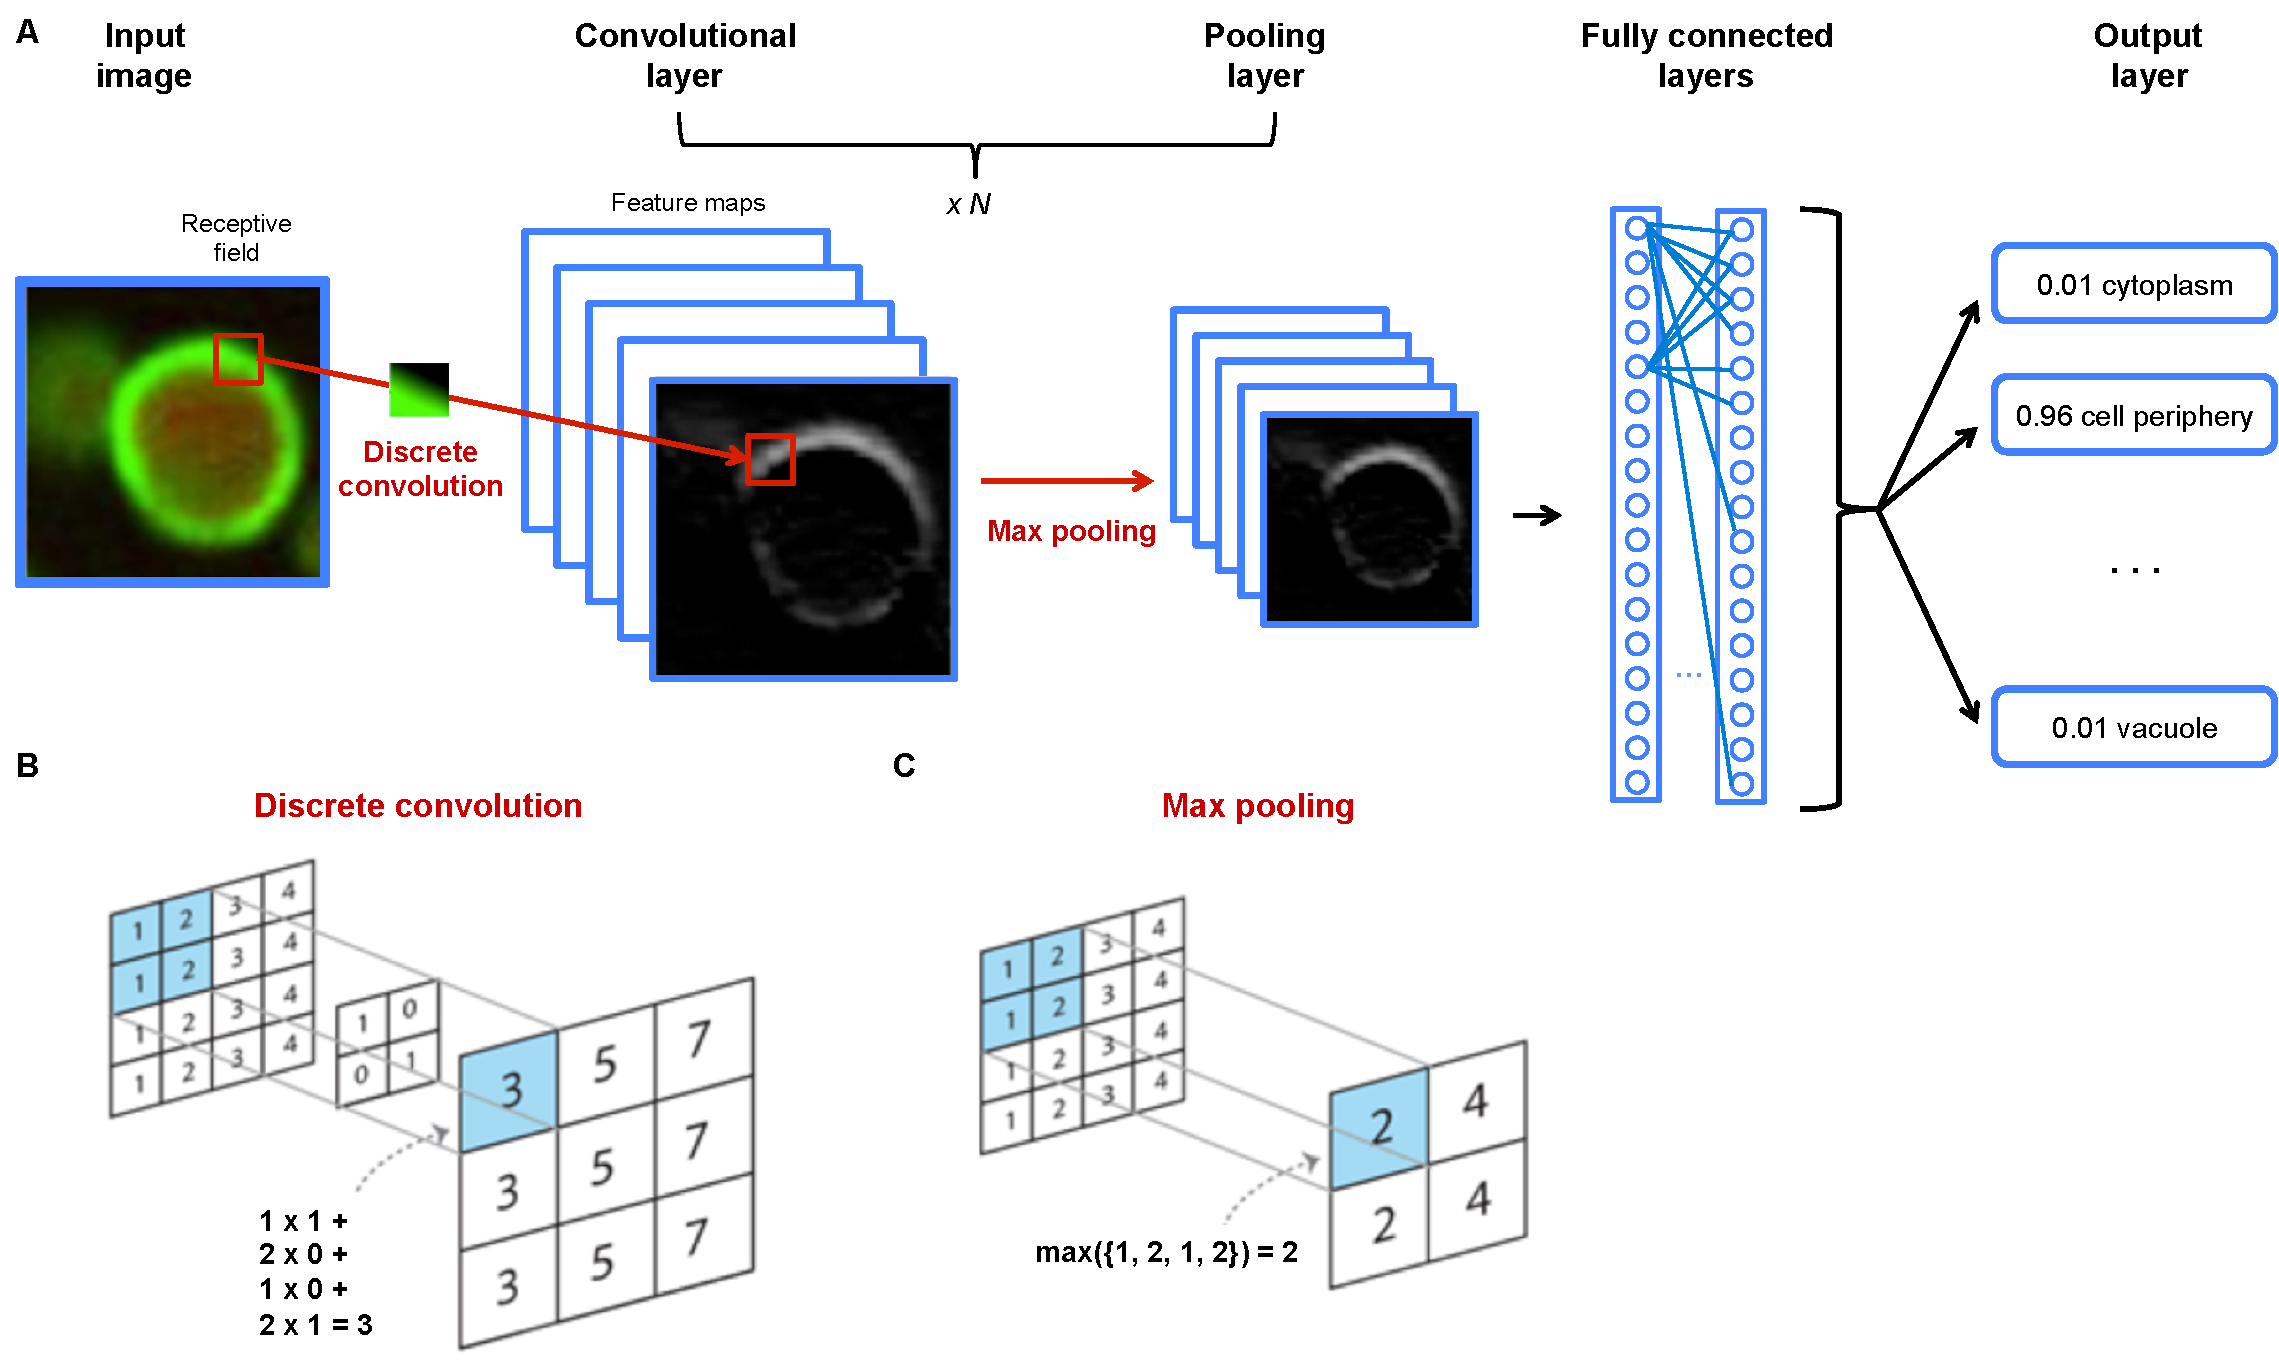
\includegraphics[width=1.0\textwidth]{figure4}
\caption[Convolutional neural networks (CNN).]{Convolutional neural networks (CNN). (A) A typical CNN consists of a number of convolutional and pooling layers, two fully connected layers, and one output layer. Each convolutional layer consists of multiple feature maps, with neurons responding to a particular feature in a receptive field (red square). One feature map responding to the membrane of a cell at a particular angle is highlighted on the edge. (B) Neuron activities result from a discrete convolution of their receptive field. (C) Max pooling computes the maximum neuron activity over a small patch, reducing the dimension of a convolutional layer.}
\label{fig:figure4}
\end{figure}
